% !TeX spellcheck = en_US
\addsection{What to Play}{\images/forgetfulness.png}

\begin{multicols}{2}

Follow these suggestions if you're not sure which Scenario is best for you.

\subsection*{Cooperative Mode}

If you're new to the game and want to try \textbf{learning the rules}, start with \pagelink{Emerald Island}{Emerald Island}.
For a big adventure for \textbf{up to 6 players} with an epic battle at the end, try \pagelink{Titans' Stronghold}{Titans' Stronghold}.
For more tactical play for two players, try \pagelink{Sentinels}{Sentinels}.

\subsection*{Clash Mode}

If you'd like to play a 2- or 4-player ``capture the Grail'' Scenario with interesting twists, try \pagelink{Bloody Grail}{Bloody Grail}.
For an exciting boss fight for 2-3 players, choose \pagelink{The Hunt}{The Hunt}.
For an inevitable epic battle between two players with a possible siege, play \pagelink{Dragoncurse Castle}{Dragoncurse Castle}.

\subsection*{Campaign}

There is a 3-Scenario Inferno \pagelink{1. A Devilish Plan}{Dungeons and Devils} Campaign at the end if you prefer solo play.

\subsection*{Recommendations}

For information regarding your play time, strategizing, and custom rules, checkout out \pagelink{Recommendations}{Recommendations} at the and of this book.

\end{multicols}

\iftoggle{printable}{
  \enlargethispage{2\baselineskip}
}{}

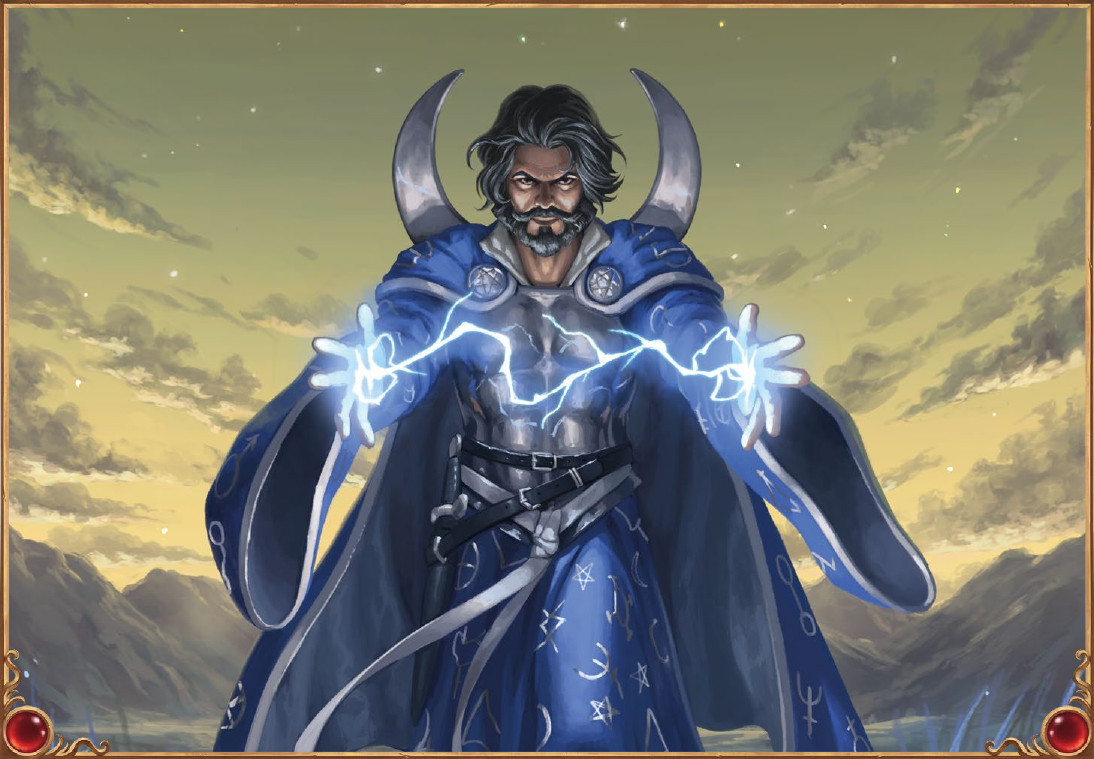
\includegraphics[width=\linewidth]{\art/enchanter.jpg}

\vspace*{-1em}
